\documentclass[12pt]{scrartcl}

\usepackage[T1]{fontenc}
\usepackage[ngerman]{babel} % Silbentrennung
\usepackage[utf8]{inputenc} % Umlaute
\usepackage{graphicx}
\usepackage[style=authortitle-icomp]{biblatex}
\usepackage[babel,german=guillemets]{csquotes}

\usepackage{xcolor}
\definecolor{dark-red}{rgb}{0.4,0.15,0.15}
\definecolor{dark-blue}{rgb}{0.15,0.15,0.4}
\definecolor{medium-blue}{rgb}{0,0,0.5}

\usepackage{hyperref}
\hypersetup{
    colorlinks, linkcolor={dark-red},
    citecolor={dark-blue}, urlcolor={medium-blue}
}


\begin{document}



%%%%%%%%%%%%%%%%%%%%%%%%%%%%%%%%%%%%%%%%%%%%%%%%%%%%%%%%%%%%%%%%%%%%%%%%%%%%%

% Deckblatt
% Fehlt noch WS 13/14

\begin{titlepage}

\begin{center}


\includegraphics[width=1.0\textwidth]{fhkoeln.jpg}
\\[2cm]
\textsc{\LARGE EIS}
\\[0.2cm]
{\Large Entwicklung Interaktiver Systeme}
\\[3cm]
\textsc{\Huge Konzept}

\vfill

\textsc{\Large Team}\\
Duc Duy Khuong (11084720)\\
Robert Kellermann (11082910)
\\[1cm]
\textsc{\Large Betreuer}\\
Prof. Dr. Kristian Fischer\\
Prof. Dr. Gerhard Hartmann\\
Renée Schulz\\
Christopher Messner
\\[2cm]
\today

\end{center}

\end{titlepage}

\tableofcontents

\newpage

%%%%%%%%%%%%%%%%%%%%%%%%%%%%%%%%%%%%%%%%%%%%%%%%%%%%%%%%%%%%%%%%%%%%%%%%%%%%%

\section{Einführung}

Musik spielt bei vielen Menschen im alltäglichen Leben eine wichtige Rolle. Ob man Musik hört oder selber ein Instrument spielt, ist da jedem selber überlassen. Diejenigen, die sich sich für Letzteres entscheiden, wollen dann meistens auch mit anderen Musikern zusammen Projekte starten und gründen eine Band.

Die Organisation der Band spielt dabei eine übergeordnete Rolle, denn die Bandproben hängen vom Zeit- und Ortsfaktor ab, wann hat Jeder Zeit und wo wird der Bandraum sein. Wenn diese Fragen geklärt sind, besteht die Absicht darin, die Zeit der Probe so effizient wie möglich zu nutzen.

%% vielleicht noch etwas ausführlicher?

\subsection{Problem}

Ein grundlegendes Problem ist der Umgang mit neuen Ideen. Wenn beispielsweise ein Musiker eine Idee zu einem neuen Song hat, etwa ein Riff oder eine kurze Melodie, muss er bis zur nächsten Probe warten, um sie der Band vorzustellen. Zu dieser Idee steuern die anderen Musiker dann meist ihre Ideen bei und entwickeln somit gemeinsam einen neuen Song. Dieser kreative Prozess nimmt jedoch viel Zeit in Anspruch. Aufgrund der wertvollen Zeit im Proberaum entsteht somit ein Druck auf den Bandmitgliedern und der Kreativität der Musiker wird möglicherweise kein freier Lauf gelassen.

\subsection{Idee}

Um diesen Zeitdruck beim Komponieren im Proberaum zu vermeiden, wäre es hilfreich, neue Ideen auch außerhalb der Bandproben festzuhalten und mit den Bandkollegen zu teilen. Ein Austausch von Ideen und das Beitragen von Einfällen und weiteren Ideen dazu könnte entweder alleine in Ruhe oder in Kommunikation mit den anderen Bandmitgliedern über das Internet erfolgen. Dadurch könnte die Zeit im Proberaum für das tatsächliche Proben des Zusammenspiels in der Band und den letzten Schliff an neuen Songs genutzt werden, während die kreativen, meist sehr zeitaufwändigen Kompositionsprozesse außerhalb der Proberaumatmosphäre stattfinden.

%%%%%%%%%%%%%%%%%%%%%%%%%%%%%%%%%%%%%%%%%%%%%%%%%%%%%%%%%%%%%%%%%%%%%%%%%%%%%

\section{Ziele}

In dieser Zielhierarchie soll deutlich gemacht werden, welche kurz- und langfristigen Ziele das Projekt \emph{CoMusic} ausmachen. Danach soll dann in der Zielpriorisierung aufgezählt werden, welche dieser Ziele die Besonderheiten und die Alleinstellungsmerkmale des Projektes darstellen.
% Einführung zu den Zielen vllt noch etwas ausführlicher? Zielpriorisierung besser erklären?

\subsection{Strategische Ziele}

% zu wenig Ziele definiert
% ausformulieren, detaillierter, mehr eingehen und verschärfen
\begin{itemize}


\item Der Zeitdruck, der bei kreativer Arbeit an neuen Songideen auftritt, kann vermieden werden. Der begrentze Faktor Zeit soll eine verminderte Rolle spielen
\item Aufkommende Ideen oder Einfälle sollen in Ruhe festzuhalten sein
\item Aktivitäten einer Band, die sonst während der Proben durchgeführt werden, sollen außerhalb ermöglicht werden
\end{itemize}

Langfristiges Ziel des Systems soll sein, alle beeinträchtigenden Aspekte, die beim gemeinsamen musizieren entstehen können, zu verringern. Es wird versucht die Aktivitäten auch auf außerhalb der Proben zu verlagern und zu erleichtern, damit effizienter gearbeitet werden kann.

\subsection{Taktische Ziele}


\begin{itemize}
\item gemeinsam nutzbare Plattform
\item Das Teilen und Ausarbeiten von Songideen soll in Ruhe außerhalb des Proberaumes geschehen können
\item Unabhängiges Arbeiten voneinander
\item Kommunizieren der Bandmitglieder über Ideen soll möglich sein
\
\end{itemize}

Taktisches Ziel ist die Entwicklung eines Systems, das Musikern eine gemeinsam nutzbare Plattform gibt, welche die Funktion bereitstellt gemeinsam an Kompositionen arbeiten zu können. Dabei steht nicht in Vordergrund wo und wann dies geschehen soll, sondern viel mehr, dass es überall möglich ist. Das Erstellen und Bearbeiten von Kompositionen ist unabhängig voneinander und geschieht außerhalb des Proberaumes. 
Zudem ist die Kommunikation dabei ein wichtiger Aspekt, die einzelnen Mitglieder können sich über Ideen austauschen und diese kommentieren oder ähnliches.
% Kollaborativ ist zu wolkig -> mehr spezifizieren

\subsection{Operative Ziele}

Um die strategischen und taktischen Ziele zu erfüllen werden zunächst geeignete Vorgehens- und Gestaltungsmethoden der Mensch-Computer-Interaktion ausgewählt. Darauf hin werden die technischen Anforderungen des Systems festgelegt und schließlich ein Prototyp entwickelt, welches die Funktionalitäten des System demonstriert.

\begin{itemize}
\item Vorgehensmodelle und Gestaltungsmethoden der MCI auswählen
\item Festlegung der technischen Anforderungen
\item Entwicklung eines Prototyps 
\end{itemize}

%% to add: echtzeitkommunikation, übertragene daten: änderungsinformationen, neue kommentare

\subsection[Geplante Funktionalitäten]{Geplante Funktionalitäten des Systems}

\begin{itemize}
\item Band- und Musikerverwaltung (einzelne Accounts für die Musiker, gemeinsamer Bereich für die jeweiligen Bands
\item kollaboratives Arbeiten an MIDI-Spuren innerhalb einer Kompositionsidee
\item Echtzeitaktualisierung der Spuren
\item kompositionsbezogene Kommunikation der Bandmitglieder (Chatroom, Notizen o.Ä.)
\item Optional: Generierung von Notenblättern und Tabulaturen anhand der MIDI-Dateien
\item ------------------------------
\item Band- und Musikerverwaltung
\item Zusammenarbeit an einer Kompositionsidee 
\item Ermöglichung der Echtzeit-Zusammenarbeit trotz örtlicher Unabhängigkeit
\item Option: Generierung von Musikblättern mit einheitlicher Musiknotation
\end{itemize}


%% SCHWERPUNKT auf echtzeitkollaboration !!!



% geplante Funktionalitäten: zu technisch
% Zielpriorisierung textuell formulieren, zu ungenau
% zu ungenau: Begründung warum MIDI

%% Hier evtl zusammenfassung als tabelle

%%%%%%%%%%%%%%%%%%%%%%%%%%%%%%%%%%%%%%%%%%%%%%%%%%%%%%%%%%%%%%%%%%%%%%%%%%%%%

\section{Mensch-Computer-Interaktion}

zu allgemein, nicht projektbezogen, besser darlegen
Stakeholderanalyse noch spezifischer, Grundlage für Begründungen
wirkt vorgegriffen/zusammengewürfelt

\subsection{Abwägung Nutzerzentrierte/Nutzungszentrierte Gestaltung}
Um eine geeignete Grundlage zu schaffen, damit eine erfolgreiche Umsetzung des System erfolgen kann, sollte eine vollständige und durchdachte Planung stattfinden. Dazu zählt die Konzeptionierung, Evaluation, Gestaltung und die Entwicklung. 
Mit Hilfe verschiedener Vorgehensmodelle und Methoden der Mensch-Computer-Interaktion ist es möglich dies zu realisieren.

Erste zentrale Frage ist es, festzustellen welche der beiden Möglichkeiten, benutzerzentrierte oder benutzungszentrierte Gestaltung, bei der Entwicklung des Systems sinnvoller ist.

Aus der Problematik bzw. der Motivation, lässt sich ableiten, dass die Entwicklung der Anwendung der Intention dient, dass die Bedüfnisse der Benutzer also die “user needs” erfüllt werden und daraus folgend eine gute “user experience” zu erreichen. 
In dem Fall sind die Benutzer, die im Hauptfokus des Projekts stehen, die Musiker, speziell die in Gruppen wie Bands etc., was bedeutet, dass das System auf die eine Zielgruppe zugeschnitten werden muss. Auch der Nutzungskontext lässt sich daraus ableiten, wodurch sich eine benutzerzentrierte Gestaltung anbietet. Die Anforderungen der Benutzer können herauskristallisiert werden wodurch das System weitesgehend angepasst werden kann.

Dadurch sollten sie möglichst auch ohne jegliche Vorkenntnisse, bis auf die in unserem spezifischen Nutzungskontext erforderten, mit dem System interagieren können.
Um dies gewährleisten zu können ist es notwendig, die Gebrauchstauglichkeit des Systems zu maximieren, d.h. die Entwicklung und Gestaltung. Alles, was ihn in der Interaktion mit dem System beeinträchtigen könnte, sollte möglichst vermieden werden. Im Gegenteil, die Anwendung sollte den Benutzer in der Verwendung unterstützen können. Dazu zählt z.B. eine nicht zu komplexe grafische Benutzeroberfläche (GUI). Die Elemente der GUI sollten so gewählt sein, dass die Gebrauchstauglichkeit hoch ist keine Verwirrung oder Überforderung stattfindet.


\subsection{Auswahl der MCI-Methoden}

Nach der Wahl des Vorgehensmodells, werden einige Methoden der Mensch-Computer-Interaktion ausgewählt, die Informationen liefern können, welche relevant für die Entwicklung des Systems sein können.
Diese Methoden kann man in 4 Bereiche einteilen, die sich auch im Vorgehensmodell widerspiegeln:
Die Nutzungskontextanalyse
Die Benutzermodellierung
Schnittstellendesign und die
Evaluation

\subsubsection{Nutzungskontextanalyse}

Zur Nutzungskontextanalyse gehört zunächst einmal die Festlegung der Nutzungskontexte, also wofür wird das System benötigt und in welchem Fall wird es verwendet. Dazu können Szenarien und Use Cases erstellt werden um bestimmte Kontexte untersuchen zu können. Zuvor sollte jedoch die Benutzermodellierung stattfinden, damit diese vollständig umgesetzt werden.

\subsubsection{Benutzermodellierung}

Unter die Benutzermodellierung gehört das Erstellen von User Profiles, Personae oder auch die Befragung potentieller Benutzer. 

\subsubsection{Schnittstellendesign}

Sind die Nutzungsanforderungen festgelegt, so ist der nächste Schritt die Gestaltungslösung zu entwickeln. Diese können in Form von papier-basierten Prototypen, erste digitale Mockups oder Ähnliches auftreten.

\subsubsection{Evaluation}

Als finaler Schritt, findet die Evaluation statt, d.h. es wird geprüft, ob in dieser Phase die “User Needs” zufriedenstellend erfüllt sind. Falls die Evaluation der Gestaltungslösung positiv ausfällt, kann mit der Umsetzung begonnen werden, ist dies jedoch nicht der Fall, so kann mit Hilfe Iteration, die Aspekte erneut untersucht werden, die noch zu optimieren sind.





Im weiteren Verlauf werden nun die einzelnen Schritte des Vorgehensmodells durchgegangen und die dazu passenden Methoden angewendet um eine geeignete Gestaltungslösung erstellen zu können.

%%%%%%%%%%%%%%%%%%%%%%%%%%%%%%%%%%%%%%%%%%%%%%%%%%%%%%%%%%%%%%%%%%%%%%%%%%%%%

\section{Kommunikationsablauf}

% Kommunikationsmodell abstrakter (wer mit wem, welche Inhalte, syn/asyn, welche Wege/Alternativen)
% technisch zu konkret, auf einer höheren Ebene argumentieren (Echtzeitkommunikation statt Chatroom)

- wer mit wem
- welche inhalte
- paradigmen syn/asyn
- welche wege (alternativ: peer to peer)
BEGRÜNDEN!

Im Folgenden soll die Kommunikation im System CoMusic erläutert werden. Diese ist in \ref{fig:kommunikationsmodell} dargestellt.

\begin{figure}
\centering
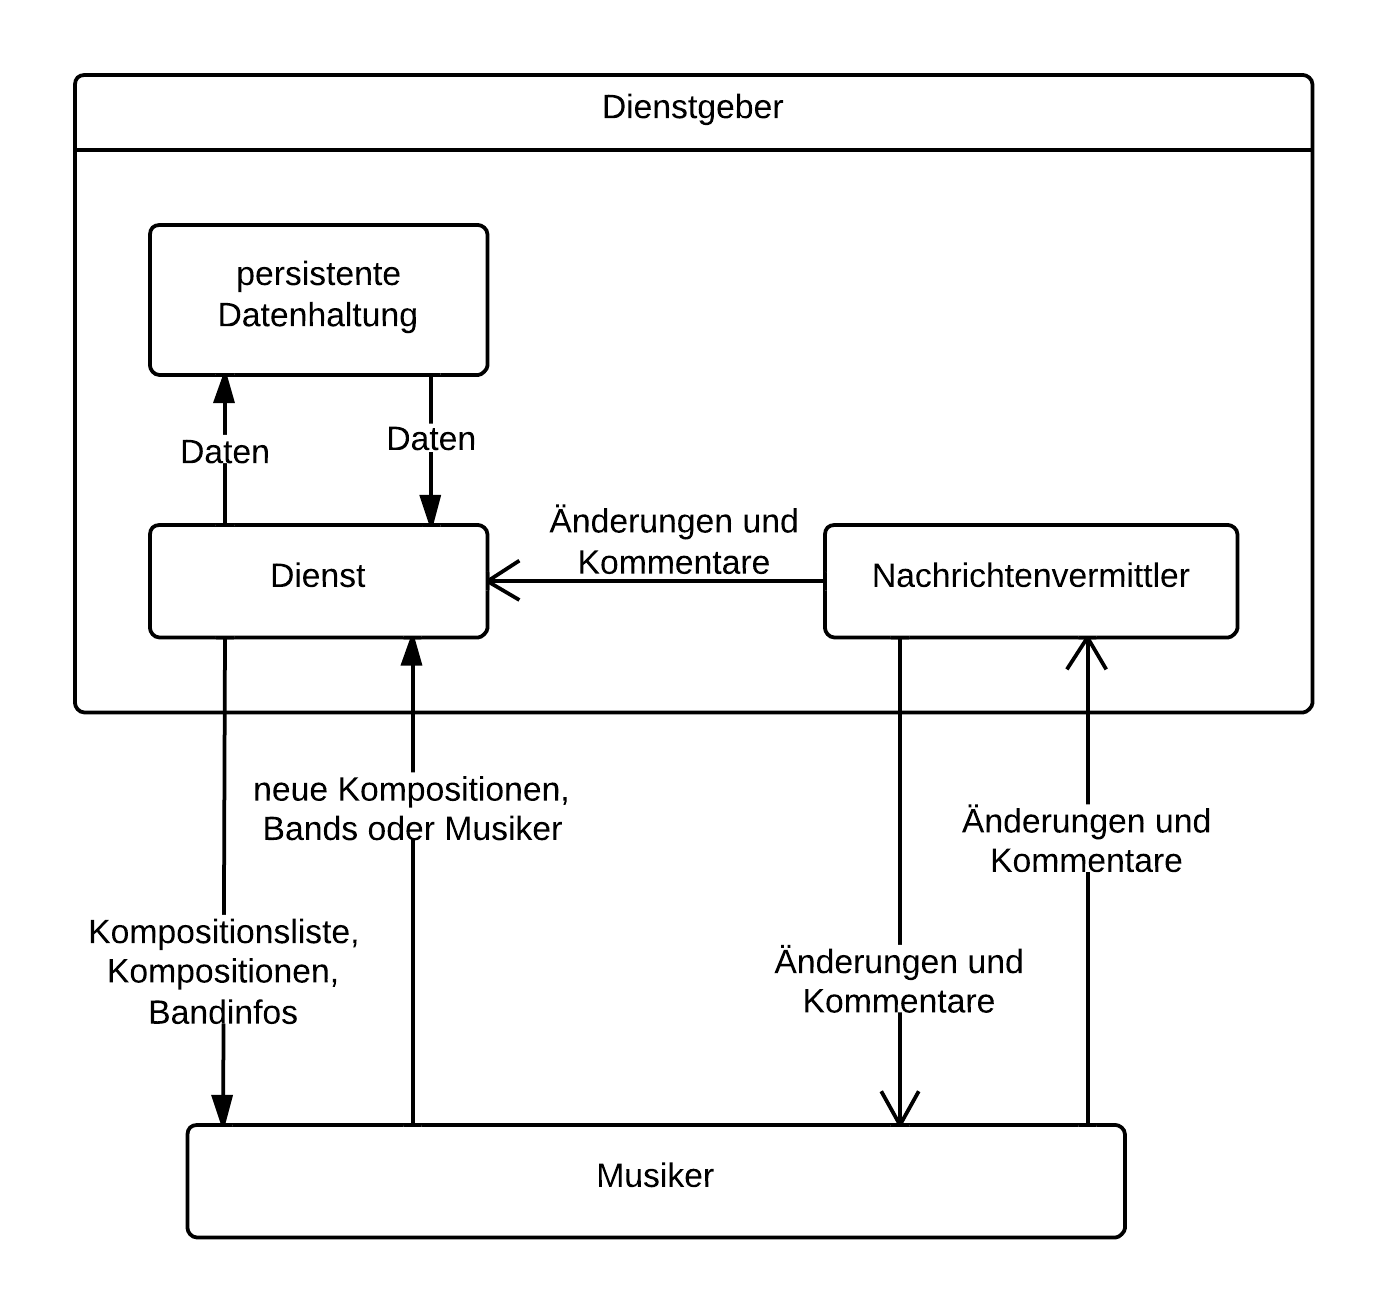
\includegraphics[scale=.25]{figures/kommunikationsmodell}
\caption{Kommunikationsmodell}
\label{fig:kommunikationsmodell}
\end{figure}

Um die Sicherheit der persistenten Daten zu gewährleisten, soll Kommunikationsteilnehmern des Systems in keinem Fall der direkte Zugang zur Datenhaltung ermöglicht werden. Dies erfolgt immer über den Dienstgeber, damit Anfragen und Daten validiert werden können. Die Kommunikation zwischen Dienst und der persistenten Datenhaltung erfolgt synchron, da es sich hier um Anfrage und Rückgabe beziehungsweise Modifizierung von Daten handelt.

Musiker können mit dem Dienstgeber kommunizieren, um etwa neue Bands, neue Musiker oder neue Kompositionen zu erstellen. Außerdem können Sie Informationen zu ihren Bands, deren Kompositionen und bestimmte Kompositionen vom Dienst anfragen. Diese Kommunikation erfolgt nach dem synchronen Request-Response Paradigma.

Die wichtigste Kommunikation ist der Austausch von Änderungsinformationen an Kompositionen und Kommentaren in Echtzeit. Diese Informationen werden von einem Nachrichtenvermittler entgegengenommen und nach dem asynchronen Publish-Subscribe Paradigma an alle aktiven Teilnehmer Teilnehmer gesendet. Ein weiterer Teilnehmer ist der Dienstgeber, der als Zuhörer fungiert und alle Änderungsinformationen in der persistenten Datenhaltung abspeichert.

Eine Alternative zum Publish-Subscribe Paradigma wäre das Peer-to-Peer Paradigma, bei welchem Änderungsinformationen von einem Teilnehmer zu allen anderen aktiven Teilnehmern gesendet würden. Dieses wird hier jedoch nicht gewählt, da es viele Nachteile birgt:
\begin{itemize}
\item Alle Teilnehmer müssen sich gegenseitig kennen
\item Bei einer Änderung entsteht beim Autor je nach Anzahl der aktiven Teilnehmer viel Datenverkehr
\item Schlecht skalierbar
\end{itemize}

%%%%%%%%%%%%%%%%%%%%%%%%%%%%%%%%%%%%%%%%%%%%%%%%%%%%%%%%%%%%%%%%%%%%%%%%%%%%%

\section{Systemarchitektur}

% Paradigmen kommen aus der Architektur nicht deutlich hervor, Paradigmen nicht mischen
% von Kommunikationsmodell zur Systemarchitektur führen
% Systemarchitektur konkreter, etwaige Softwarekomponenten, Logik der Komponenten (abstrakt)

% Zielplattform

% Vorgabe: java

\begin{figure}
\centering
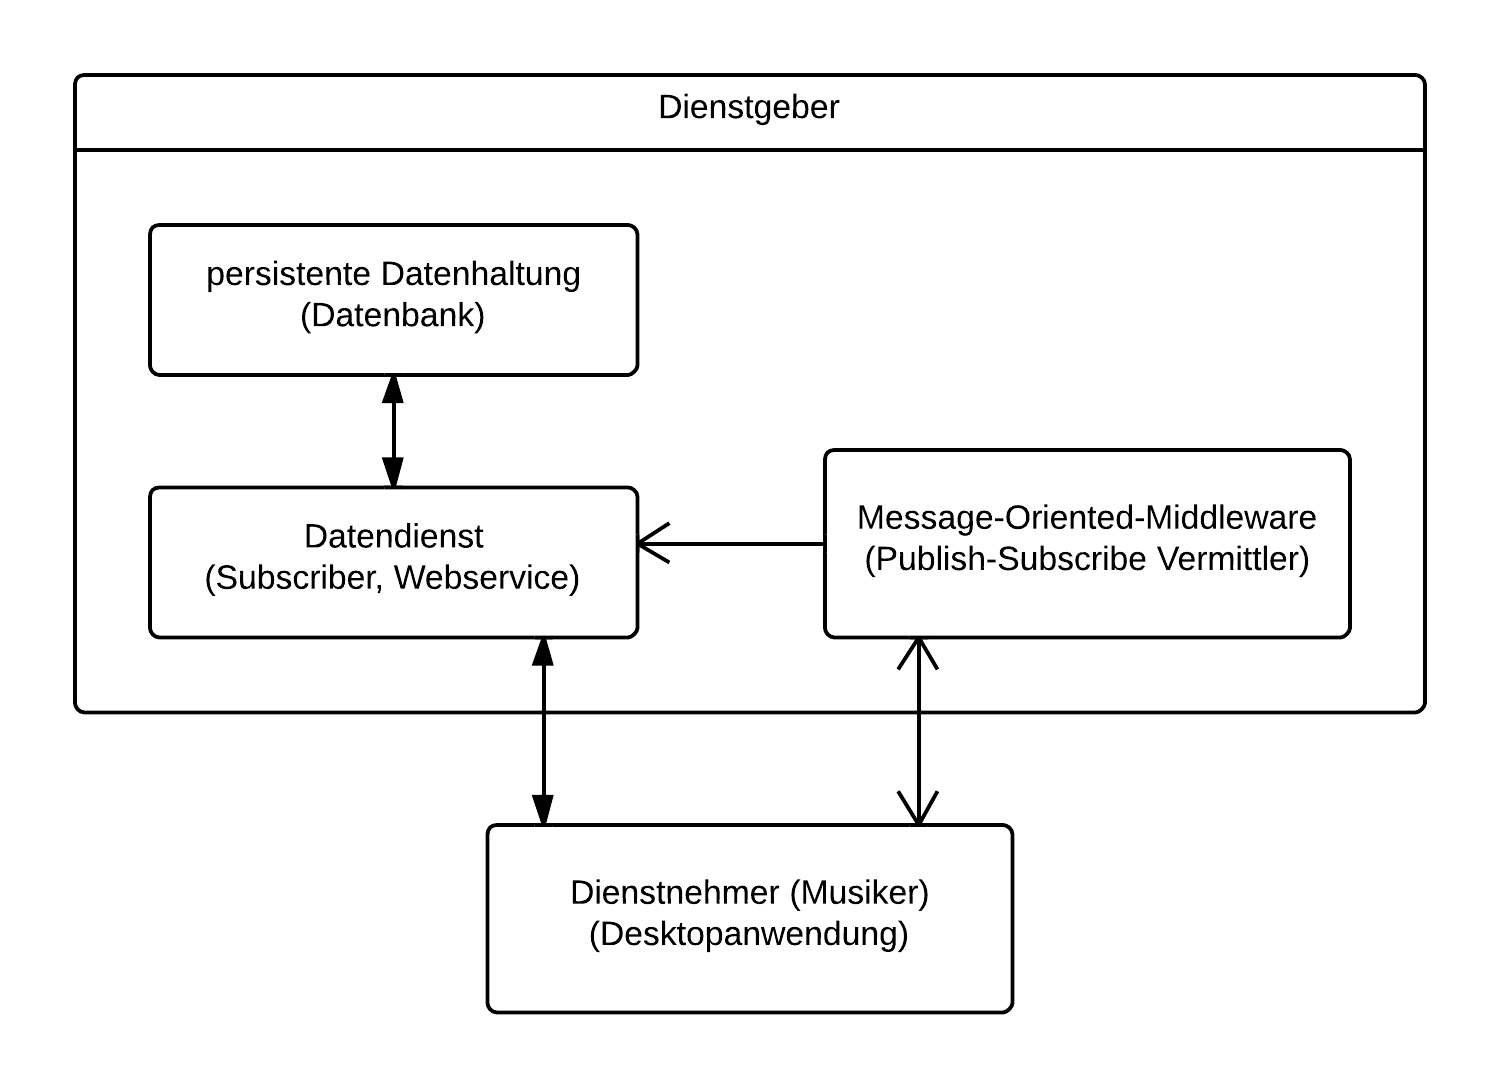
\includegraphics[scale=.25]{figures/systemarchitekturmodell}
\caption{Systemarchitekturmodell}
\label{fig:systemarchitekturmodell}
\end{figure}

Die Systemarchitektur, welche in Abbildung \ref{fig:systemarchitekturmodell} dargestellt ist, ist aus dem Kommunikationsmodell abgeleitet. Nachdem festgestellt wurde, wer mit wem wie kommuniziert, können nun die einzelnen bisher eher abstrakteren Komponenten des Systems etwas genauer beschrieben werden.

\paragraph{persistente Datenhaltung}
Die persistente Datenhaltung wird aus einer Datenbank bestehen, in der alle Daten abgespeichert werden. Welche Daten hier abgespeichert werden sollen, wird im Datenmodell (hier Referenz) beschrieben.

\paragraph{Dienst}
Der zentrale Dienstgeber hat mehrere Aufgaben.
\begin{itemize}
\item Er fungiert als Vermittler zwischen allen Systemkomponenten und der Datenbank und validiert Anfragen und Daten.
\item Er stellt einen Webservice bereit, um Dienstnehmern das Anfragen und Modifizieren von Daten zu ermöglichen.
\item Er ist Subscriber (Zuhörer) der Message-Oriented-Middleware und erhält alle veröffentlichten Informationen, um Sie in der Datenhaltung persistent zu speichern.
\end{itemize}

Durch das direkte Speichern aller Echtzeitinformationen in der persistenten Datenhaltung erhalten alle neuen Teilnehmer immer den aktuellen Stand. Andererseits können aktive Teilnehmer jederzeit das System verlassen, ohne ungespeicherte Änderungen zu hinterlassen.

% alter text

Die Grundidee besteht aus dem Kollaborieren von verschiedenen Musikern an einer Komposition in Echtzeit. Der aktuelle Stand einer Komposition soll aber auch persistent für alle Mitkomponisten gespeichert werden, damit die gleichzeitige Anwesenheit aller Benutzer nicht verpflichtend ist. So kann zum Beispiel der Gitarrist zusammen mit dem Bassisten der Band eine Idee entwerfen, zu der der Schlagzeuger später alleine seine Ideen beiträgt, ohne dass alle Beteiligten zur gleichen Zeit online sein müssen.
Eine Message Oriented Middleware agiert hier als Vermittler der Nachrichten zu Änderungen an einer Komposition. Aktive Dienstnehmer senden und empfangen diese Nachrichten im Falle von Änderungen. Der Dienstgeber der Daten empfängt diese Änderungen ebenfalls und speichert sie zu der jeweiligen Komposition persistent in einer Datenbank. Wird ein neuer Teilnehmer aktiv, holt er zunächst die aktuelle Komposition vom Dienstgeber der Daten und empfängt ab dann alle neuen Änderungen über die MOM.
Der Chatroom Dienstgeber verwaltet Chaträume für jede Komposition, sodass eine kompositionsbezogene Kommunikation zwischen den aktiven Teilnehmern einer Komposition möglich ist.
Eine klassische Benutzerauthentifizierung ermöglicht eine Zuordnung der Benutzer zu Bands und Kompositionen.

%%%%%%%%%%%%%%%%%%%%%%%%%%%%%%%%%%%%%%%%%%%%%%%%%%%%%%%%%%%%%%%%%%%%%%%%%%%%%

\section{Datenmodell}

% Datenmodell unbegründet, umstrukturieren


% alter text

Das System ist spezialisiert für die kollaborative Arbeit an Kompositionsentwürfen in Bands. Es soll von Musikern und deren Bands genutzt werden. Für jeden Musiker werden seine Anmeldedaten gespeichert. Ein Musiker kann einer oder mehreren Bands angehören. Jeder Band werden die zugehörigen Kompositionen zugeordnet. Zu einer Komposition gehören mehrere Spuren, welche jeweils eine Matrix mit den gesetzten Tönen beinhaltet. Weitere Informationen wie Abspielgeschwindigkeit und Art der Instrumente werden in den Daten für Kompositionen und Spuren festgehalten. Diese Daten werden persistent in einer Datenbank gespeichert, um sie unabhängig von den Dienstnehmern an einem Ort dauerhaft verfügbar zu machen.
Weitere Daten sind die Änderungsdaten, welche im Falle einer Änderung an einer Komposition durch einen Benutzer sowohl an alle anderen gerade aktiven Mitkomponisten als auch an den Dienstgeber der persistenten Datenspeicherung übermittelt werden.
Zunächst nicht näher behandelt werden die Kommunikationsdaten in den kompositionsbezogenen Chaträumen, die von einem Dienstgeber eines Drittanbieters verwaltet werden.


%%%%%%%%%%%%%%%%%%%%%%%%%%%%%%%%%%%%%%%%%%%%%%%%%%%%%%%%%%%%%%%%%%%%%%%%%%%%%

\section{Proof-of-Concepts}

% Proof of Concepts abstrakter

















%%%%%%%%%%%%%%%%%%%%%%%%%%%%%%%%%%%%%%%%%%%%%%%%%%%%%%%%%%%%%%%%%%%%%%%%%%%%%

\section{Marktrecherche}

% Kein Mehrwert, kein Bezug zum Projekt
% Alleinstellungsmerkmale sind zu wenig

Für die Marktrecherche wurden Produkte und Dienste untersucht, die dem Konzept von CoMusic ähnlich sind und eine Konkurrenz darstellen könnten. Dabei wurde auf zwei verschiedene Kategorien von Produkten gestoßen, welche das Konzept von CoMusik vereint.

\subsection{kollaborative Kompositionsplattformen}

Die untersuchten Produkte dieser Kategorie ermöglichen einen Austausch von Samples oder anderen Beispielaufnahmen wie Gesang sowie Texten und vieles mehr. Es können Musikideen aufgenommen und hochgeladen und mit anderen Musikern geteilt werden. So kann jeder Musiker seine Ideen zu einem Projekt beisteuern und die Beteiligten kennen in etwa die einzelnen Ideen. Ein hörbares, zusammengesetztes Beispiel aller Ideen beziehungsweise Instrumente ist hier aber nicht möglich und eine genauere Struktur oder Notation aller Instrumente ist nicht ersichtlich. Änderungen an den aufgenommenen Spuren sind nicht direkt möglich und es gibt nur sehr wenig Spielraum für Experimente, ohne eine Spur komplett neu aufzunehmen.

% Bewertung hier?
Diese Art der Kollaboration eignet sich eventuell für unabhängige Musiker, welche gemeinsam rein über das Internet Kompositionen erstellen wollen, nicht aber für eine gute Vorbereitung der Mitglieder einer Band auf eine anstehende Bandprobe.

\begin{description}
\item[Kompoz]
Möglichkeit der Kollaboration mit fremden Personen
einzelne Instrumente/Vocals sind vorhanden
Ergänzung durch andere Mitglieder der Seite 

\end{description}


\subsection{Notationseditoren}






Kompoz (www.kompoz.com)


Sound Collabs (www.soundcollabs.com)
Suche nach Komponenten(z.B. “Suche Gesang für folgendes”)
Remix Anfragen, Möglichkeit eigene Songs zum Remix für andere bereitzustellen
Verbindung mit Musiklabels, welche nach Demos suchen (Möglichkeit für Bands “rauszukommen”)

v-band (www.v-band.de)
Reines Forum mit Dateiupload.

Rifflet (www.rifflet.com)
Plattform für das Weiterentwickeln von unfertigen und/oder aufgegebenen Songs Anderer.


Digital Musician (www.digitalmusician.net)
Eher kommerziell, Projektmithilfe wie Jobangebote


Die andere Kategorie sind Dienste oder Produkte, welche das Komponieren im MIDI-Format oder anderen Notationen ermöglicht. Dies bedeutet eine präzise Struktur und einen genauen Überblick über alle Spuren für alle Beteiligten. Ideen sind leicht für jeden Musiker änderbar und man hat einen großen Spielraum zum Ausprobieren und Experimentieren.
Im Bereich Editoren und Sequenzer für verschiedene Notationen (Noten, Tabulaturen) und auch für das MIDI-Format gibt es bereits unzählige Lösungen, welche teilweise einen sehr großen Funktionsumfang und eine komplexe Bedienung haben können. Die Palette reicht von einfachen Editoren wie NoteEdit (http://noteedit.berlios.de/) über mehrspurige Kompositionswerkzeuge wie GuitarPro bis hin zu professionellen Lösungen wie Cubase (http://www.steinberg.net/de/products/cubase/) oder Logic (http://www.apple.com/de/logic-pro/), welche neben den in diesem Kontext interessanten Funktionen noch viele andere Funktionen bieten. Aufgrund der Komplexität der meisten Produkte in diesem Bereich möchten wir an dieser Stelle die Webapplikation Inudge (www.inudge.net) hervorheben, welche wegen ihrer Simplizität unserem Konzept sehr nahe kommt.
Alle der eben aufgezählten Produkte haben einen gemeinsamen Nachteil: es ist keine einfache Kollaboration in Echtzeit möglich, lediglich das Teilen bereits notierter Ideen ist möglich.



%%%%%%%%%%%%%%%%%%%%%%%%%%%%%%%%%%%%%%%%%%%%%%%%%%%%%%%%%%%%%%%%%%%%%%%%%%%%%

\section{Geschäftsmodell}

% glaubhaft darstellen
% schon Entscheidung treffen
% Etablierung am Markt und Nutzerbasis fehlt

\subsection{mögliche Geschäftsmodelle}

Um ein solches System gewinnbringend zu vermarkten, gibt es mehrere Alternativen.

\paragraph{Lizenzen}
Als Erstes könnte man das Produkt, mit dem der Benutzer arbeitet, zu einem Festpreis verkaufen. Dies würde jedoch Bands abschrecken, da jeder Musiker für sich das Produkt kaufen müsste. Falls eine Nutzung doch erwünscht ist, würden aus finanziellen Gründen eventuell nur ein Teil der Musiker (etwa die Hauptkomponisten) das Produkt kaufen und das gemeinsame Komponente der gesamten Band wäre nicht mehr gegeben. Außerdem ist ein solches Geschäftsmodell unberechenbarer als Andere, da Lizenzen vergeben werden müssen, diese möglicherweise innerhalb der Band von mehreren Personen genutzt werden oder sogar für die Öffentlichkeit angeboten werden. Technische Funktionen für die Lizenzprüfung könnten durch illegale Modifikation der Software ausgehebelt werden und dem Geschäftsmodell schaden. Daher ist dieses Geschäftsmodell für unser Projekt eher weniger von Interesse.

\paragraph{Werbung}
Andererseits könnte man das Produkt zunächst kostenlos anbieten, jedoch (kontextbezogene) Werbung einblenden. Werbeflächen innerhalb eines Programm wirken meist allerdings sehr störend und abschreckend. Daher wäre das Einblenden von Werbung von Sponsoren aus dem Musikbereich beim Starten oder Beenden des Programmes von Werbung eine weitere Möglichkeit.

\paragraph{monatliche Gebühren}
Eine andere Möglichkeit wäre, für die Nutzung des Systems einer ganzen Band etwa monatlich Gebühren zu verlangen. So kann der Zugang zum Beispiel aus der Bandkasse finanziert werden und alle Mitglieder sind frei in der Nutzung. Es besteht also kein Ausgrenzen oder sonstiger Druck auf die Band und auch würde  störende Werbung kein Thema mehr sein.

\subsection{Geschäftsmodell für CoMusic}

Für dieses Projekt wurde eine Kombination der beiden letzten Möglichkeiten ausgewählt. Das Produkt soll also über monatliche Gebühren finanziert werden. Bezahlt wird als gesamte Band, sodass alle Mitglieder der Band das System nutzen können und die Nutzung beispielsweise aus der Bandkasse finanziert wird. Um das Produkt jedoch am Markt etablieren zu können und potentielle Nutzer nicht von Gebühren abzuschrecken, soll das Produkt einen kostenlosen Testzeitraum zur Verfügung stellen, in dem Bands das System testen und sich unverbindlich von CoMusic überzeugen lassen können.

Um das Risiko eines Misserfolges zu vermindern, soll während der kostenlosen Testphase beim Starten oder Beenden des Programmes dezente und kontextbezogene Werbung von Sponsoren aus dem Musikbereich angezeigt werden.


%%%%%%%%%%%%%%%%%%%%%%%%%%%%%%%%%%%%%%%%%%%%%%%%%%%%%%%%%%%%%%%%%%%%%%%%%%%%%

\section{Alleinstellungsmerkmal}

Wie bereits in der Marktrecherche deutlich geworden ist, schlägt unser Konzept eine Brücke zwischen den bisher unabhängigen Kategorien Kollaborierungsdienste und Notationseditoren. Insbesondere die einfache und die intuitive Bedienung für das kollaborative Entwickeln und Vorrantreiben von Kompositionsideen speziell für Bands als Vor- und Nachbereitung von Bandproben charakterisieren das Alleinstellungsmerkmal unseres Konzeptes.

%%%%%%%%%%%%%%%%%%%%%%%%%%%%%%%%%%%%%%%%%%%%%%%%%%%%%%%%%%%%%%%%%%%%%%%%%%%%%

\section{Risiken}

% alle Risiken betrachten (projektinterne Risiken)
% zu grob formuliert, Lösungsvorschläge fehlen
% Keine Struktur

%% PUNKTE

%neuer Text
Selbstverständlich bestehen bei der Bearbeitung des Projekts Risiken, die beachtet und behandelt werden müssen. Dabei gibt zum Einen die Risiken, die das Projekt an sich betreffen und zum Anderen die projektinternen, welche das Team und die Projektbearbeitung betreffen.

\paragraph{Projektspezifisch}
\begin{itemize}
\item eine stehende Internetverbindung wird für die Verwendung des Systems voraussgesetzt
\item es sind fortschrittliche musikalische Vorkenntnisse von Nöten, für die Umsetzung in MIDI
\item ggf. werden weitere Werkzeuge benötigt, die das Einspielen der Musik unterstützt (z.B. Audio-Interface,MIDI-Keyboard etc.)
\item Proof-of-Concepts könnten fehlschlagen und müssen durch Alternativen abgesichert werden.
\end{itemize}


\paragraph{Projektintern}
\begin{itemize}
\item Zeitprobleme: parallel laufende Module und Projekte nehmen ebenfalls Zeit ein; Umfang des Projektes ist sehr groß 
\item Ausfall eines Teammitgliedes: es könnte sein, dass ein Mitglied aus diversen Gründen ausfällt und das Projekt nicht weiter durchführen möchte
\item Einhaltung des Projektplanes könnte nicht wie geplant erfolgen, weil die Schätzung des Aufwandes zu gering oder zu hoch sein könnte
\end{itemize}


Ein wichtiger Lösungsansatz für die erfolgreiche Durchführung des Projektes ist die gründliche und organisierte Planung, sei es im Hinblick auf die Zeit oder auf inhaltliche Aspekte.  Außerdem ist es wichtig Alternativen zu haben, für den Fall von auftretenden Problemen, die zeitnah nicht gelöst werden können.

%%%%%%%%%%%%%%%%%%%%%%%%%%%%%%%%%%%%%%%%%%%%%%%%%%%%%%%%%%%%%%%%%%%%%%%%%%%%%

\section{Projektplan}

% Feingranularer
% Stunden schätzen
% genau einteilen wer was macht

% hier aus excel einfügen

%%%%%%%%%%%%%%%%%%%%%%%%%%%%%%%%%%%%%%%%%%%%%%%%%%%%%%%%%%%%%%%%%%%%%%%%%%%%%

\end{document}
